\chapter{مروری بر مطالعات انجام شده}\label{chap:literature_review}
  \thispagestyle{empty}
  در این فصل ابتدا مدل سیستم این پایان نامه را معرفی می‌کنیم و سپس مقالاتی را که به تخصیص منابع در شبکه اینترنت اشیاء پرداخته‌اند بررسی می‌کنیم.

  در این پایان نامه فرض می‌کنیم که تعدادی سرویس وجود دارند.
  هر سرویس، منابع داده خود مانند داده‌های حسگر‌ها و مقصد نتایج مانند فعال کننده‌های خود را دارد و می‌خواهد تابعی مشخص را روی  داده‌های خام خود اجرا کند و نتیجه به مقصد‌ها ارسال شوند.
  برای پردازش داده‌های سرویس‌ها باید منابع پردازشی به سرویس‌ها اختصاص پیدا کنند.
  مسئله تخصیص منابع در این پایان نامه به صورت یک مسئله بهینه سازی فرمول بندی شده است که تابع هدف آن کمینه کردن مجموع وزن دار هزینه سرویس‌ها می‌باشد.
  در این تابع هدف، هزینه هر سرویس، تابعی از تاخیر سرویس و نرخ پردازش داده‌های آن مدل می‌شود.

  \section{تخصیص منابع پردازشی در شبکه اینترنت اشیاء}
    مقاله \cite{sarkar2016theoretical}، یک فرمول بندی ریاضی برای پردازش مه ارائه می‌دهد.
    برای این کار اجزاء مختلف را تعریف می‌کند و به مطالعه‌ی تفاوت‌های پردازش مه با پردازش ابری مرسوم می‌پردازد.
    مدل سیستم این مقاله در \cref{fig:chapter_2:system_model_sarkar2016theoretical} رسم شده است.
    همانطور که از این شکل مشخص است، در این مقاله سیستم از سه لایه تشکیل شده است.
    در لایه اول دستگاه‌های اینترنت اشیاء قرار دارند که وظیفه جمع‌آوری داده‌های حسگر‌ها و وقایع و ارسال داده‌های خام به گره بعدی را دارند.
    لایه دوم که به عنوان لایه مه معرفی شده است از دستگاه‌هایی مانند مسیریاب‌ها و نقاط دسترسی\LTRfootnote{Access Point} تشکیل شده است که می‌توانند داده‌ها را پردازش و به صورت موقت ذخیره کنند.
    این دستگاه‌ها به چهارچوب‌های ابری متصل هستند و مسئول ارسال اطلاعات به صورت متناوب به ابر می‌باشند.
    در لایه سوم پردازش ابری قرار دارد که بالاترین لایه می‌باشد و شامل تعدادی منبع پردازشی با ظرفیت بالا می‌باشد که می‌توانند حجم زیادی از داده‌‌ها را پردازش و ذخیره سازی کنند.
    با بررسی انجام شده، پردازش مه به کمک پردازش ابری می‌تواند پاسخ گوی نیاز نسل بعدی کاربرد‌های اینترنت اشیاء باشد.
    نتایج مورد مطالعه نشان می دهند که زمانی که ۲۵٪ کاربرد‌های اینترنت اشیاء نیاز به سرویس‌های بلادرنگ با تاخیر کم دارند، استفاده از پردازش مه باعث کاهش ۴۰٫۴۸٪ در انرژی مصرفی می‌شود.
    با این حال این مقاله هیچ استراتژی بهینه سازی معرفی نکرده است.

    \begin{figure}[h]
      \centerline{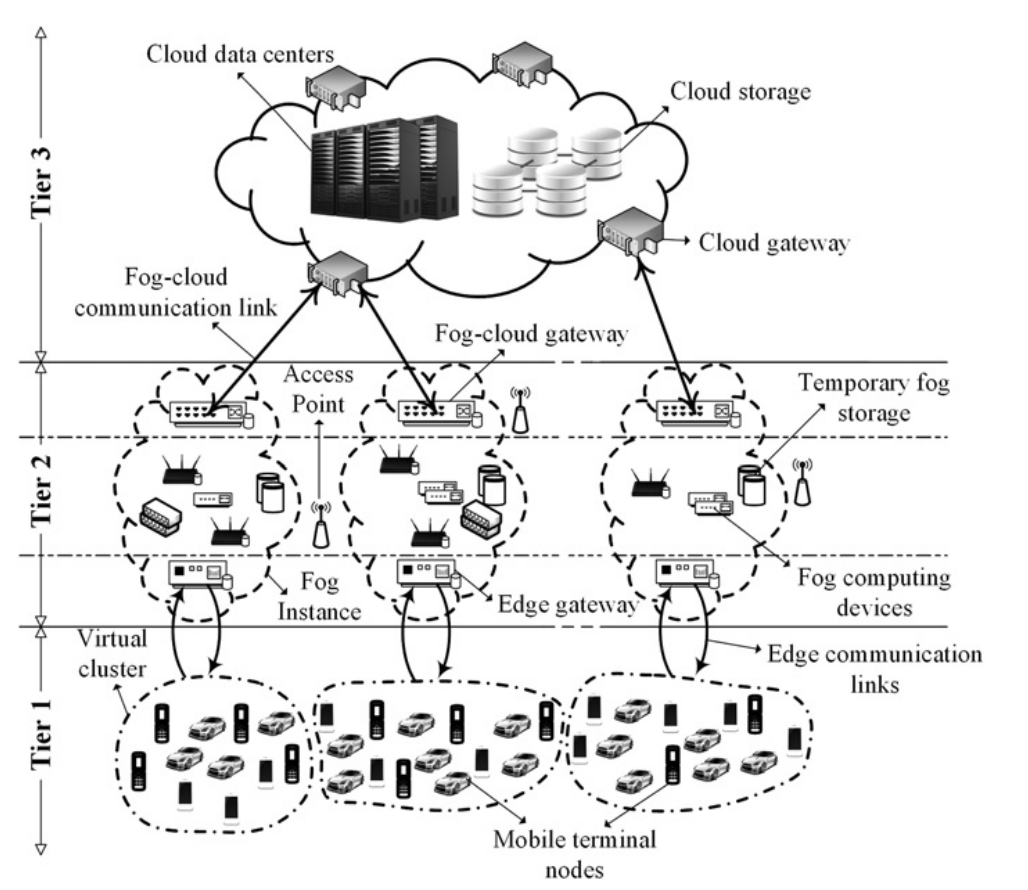
\includegraphics[width=10.5cm]{graphics/chapter_2/system_model_sarkar2016theoretical}}
      \caption{مدل سیستم مقاله \cite{sarkar2016theoretical}}
      \label{fig:chapter_2:system_model_sarkar2016theoretical}
    \end{figure}

    مقاله \cite{heng2019computing} به تخصیص منابع پردازشی در شبکه پردازشی لبه متحرک پرداخته است.
    در این مقاله بر مبنای بازی‌های پتانسیلی\LTRfootnote{Potential Game} یک راه حل برای تخصیص منابع پردازشی معرفی شده است که انرژی مصرفی را کاهش و بهره‌وری منابع پردازشی را افزایش می‌دهد.
    مدل سیستم این مقاله در \cref{fig:chapter_2:system_model_heng2019computing} آورده شده‌است.
    راه حل ارائه شده از دو بخش تشکیل شده است.
    بخش اول شامل کنترل توان با استفاده از بازی‌های پتانسیلی است و بخش دوم به تخصیص منابع پردازشی با استفاده از برنامه‌ریزی خطی می‌پردازد.
    هدف از پیدا کنترل توان، پیدا کردن مجموعه توان ‌های ارسالی ایستگاه‌های پایه\LTRfootnote{‌Base Station} است به طوری که تابع پتانسیل شبکه بیشینه شود.
    هدف تخصیص منابع پردازشی، بیشینه کردن میانگین ضریب تخصیص منابع پردازشی در شبکه با توجه به نتیجه‌ی بخش کنترل توان است.
    در مقایسه با روش‌های مرسوم، راه حل پیشنهاد شده در این مقاله بهره‌برداری منابع پردازشی و مصرف انرژی را به میزان چشمگیری بهبود می‌بخشد.

    \begin{figure}[h]
      \centerline{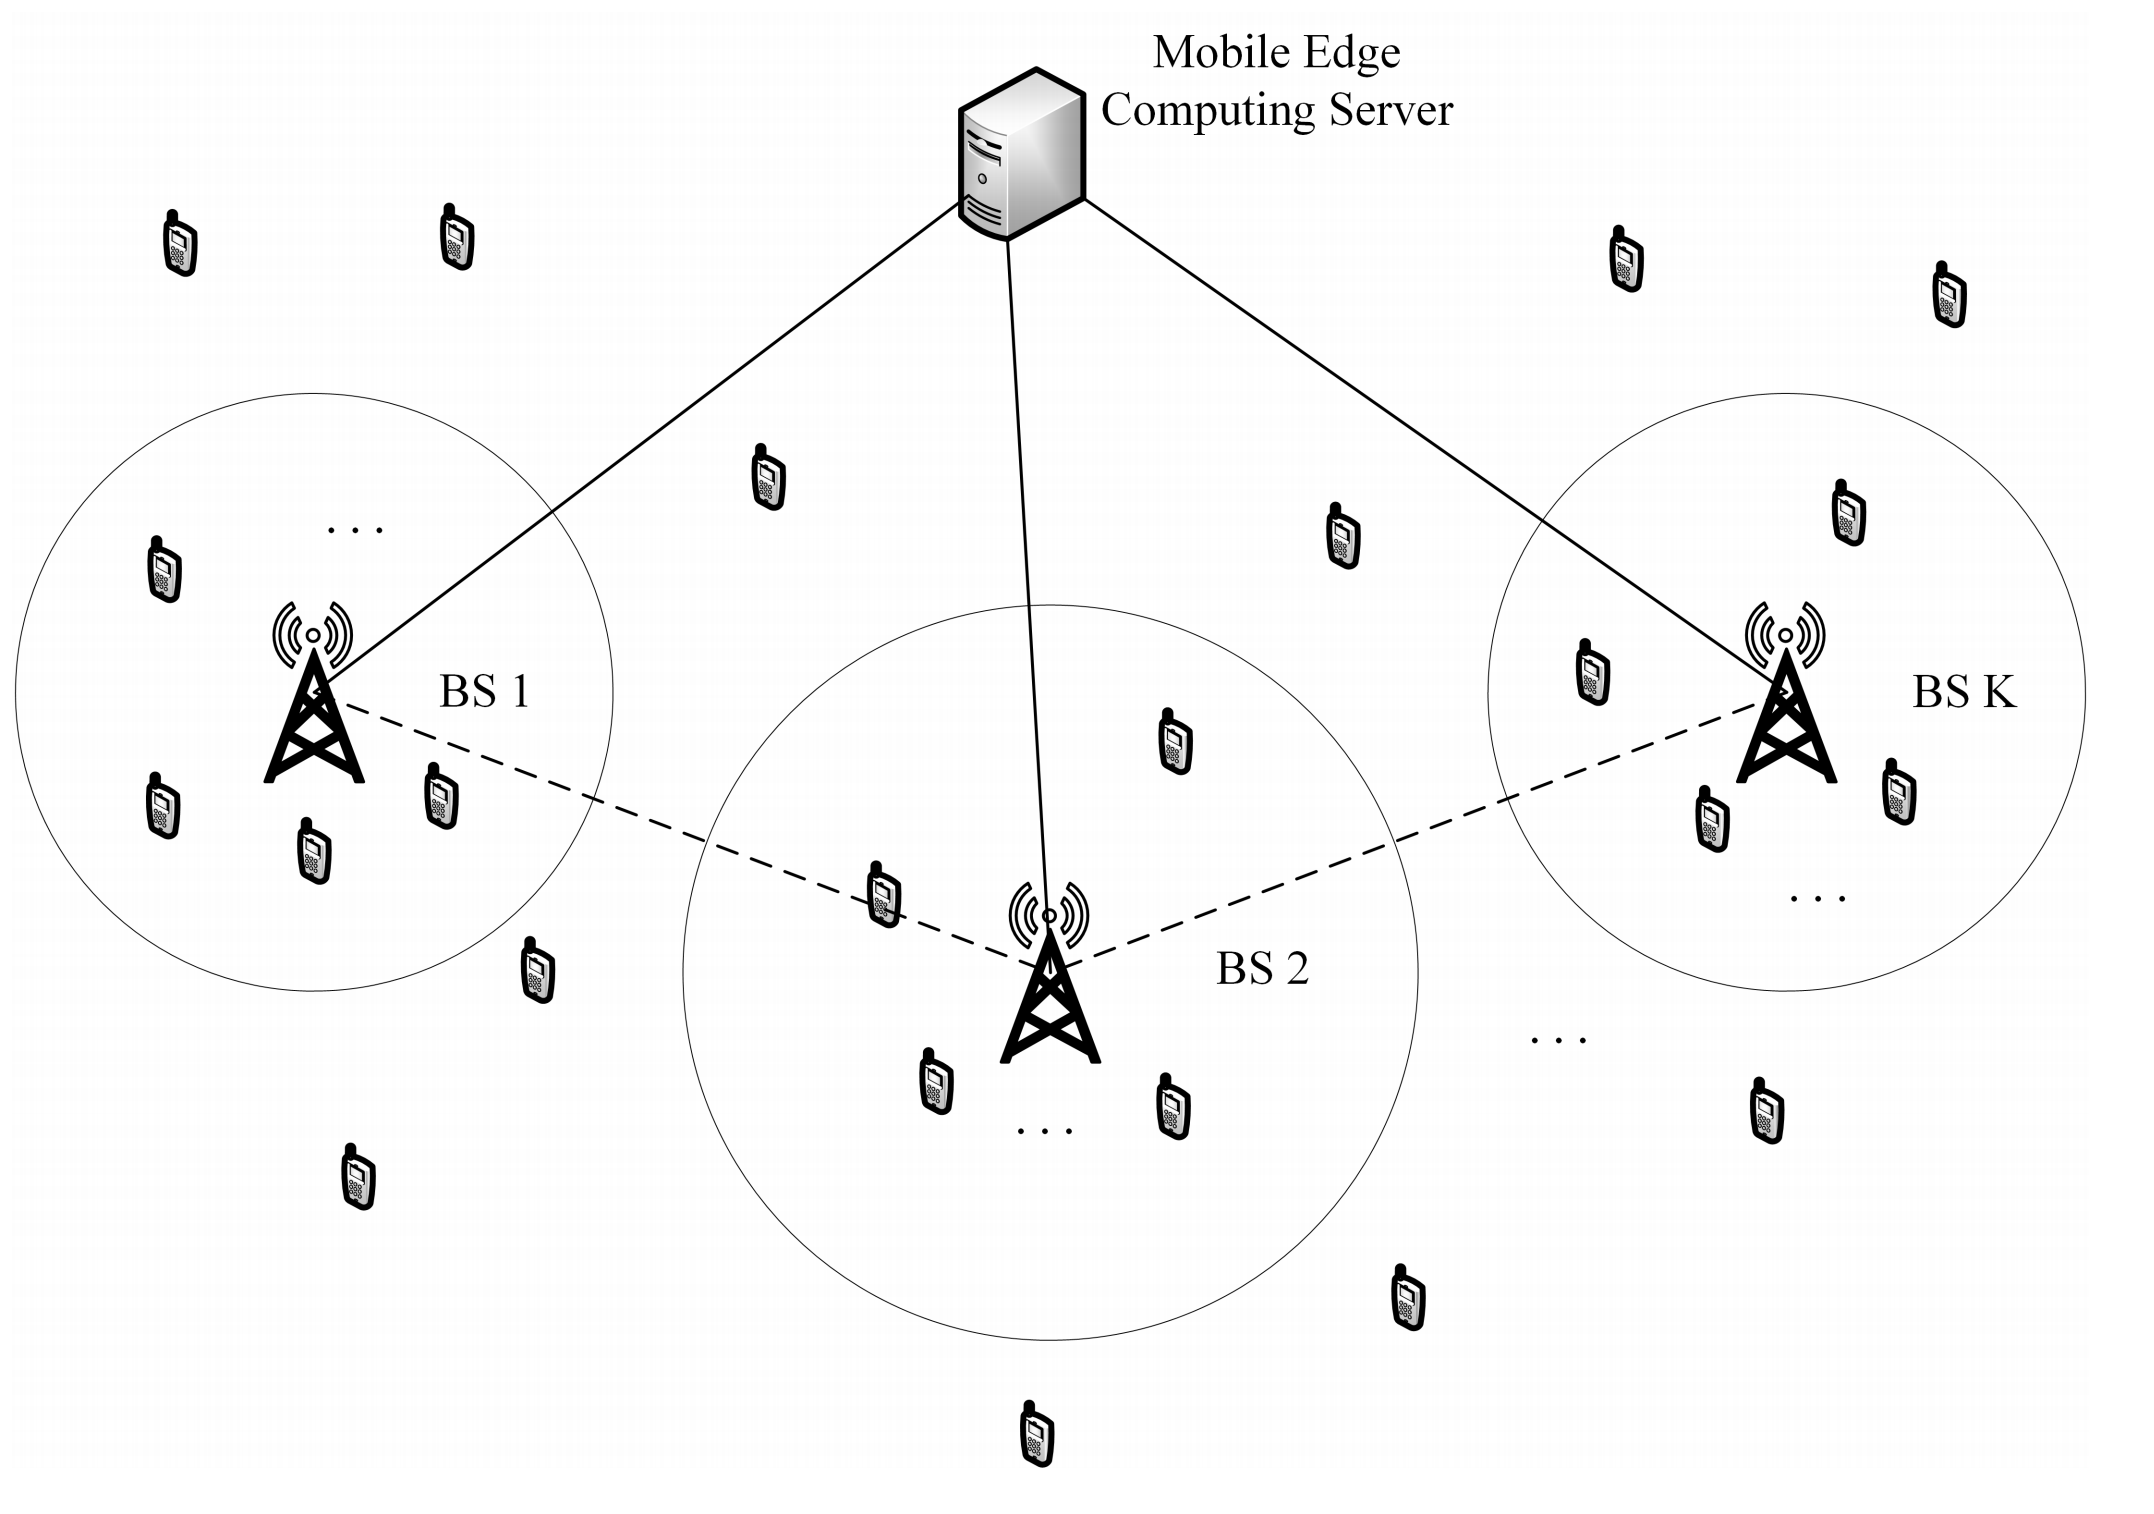
\includegraphics[width=10cm]{graphics/chapter_2/system_model_heng2019computing}}
      \caption{مدل سیستم مقاله \cite{heng2019computing}}
      \label{fig:chapter_2:system_model_heng2019computing}
    \end{figure}

    نویسندگان در \cite{deng2016optimal} چهارچوبی پیاده سازی کرده‌اند که در اختصاص منابع پردازشی در یک شبکه ابری و مه، تاخیر انتقال و مصرف انرژی را بهینه می‌کند.
    در مدل آن‌ها، لایه‌ی پردازش مه، بین لایه کاربران و لایه‌ ابر قرار می‌گیرد و به پردازش ابری کمک می‌کند تا سرویس‌هایی با تاخیر کم‌تر و نرخ پردازش بیش‌تر به کاربران ارائه دهد.
    در این چهارچوب، بررسی اثر متقابل و هم‌کاری پردازش ابری و پردازش لبه از اهمیت خاصی برخوردار است.
    نویسندگان تخصیص منابع را به صورت یک مسأله بهینه سازی فرمول‌بندی کرده‌اند که مصرف انرژی سرویس‌ها را با محدودیتی در تاخیر آن‌ها بهینه می‌کند.
    برای حل تقریبی مسئله بهینه سازی، مسئله اصلی به سه زیر مسئله‌ی مربوط به هر زیر سیستم تفکیک شده که هرکدام قابل حل می‌باشند.
    \cref{fig:chapter_2:system_model_deng2016optimal} سیستم مدل این مقاله را با چهار زیر سیستم نشان می‌دهد.
    در انتها مبتنی بر نتایج شبیه‌سازی، نویسندگان نتیجه گرفته‌اند که با کاهش استفاده از بخشی از منابع پردازشی برای کاهش پهنای‌باند مورد نیاز و کاهش تاخیر انتقال، پردازش لبه به صورت چشمگیری کارایی پردازشی ابری را افزایش می‌دهد.

    \begin{figure}[h]
      \centerline{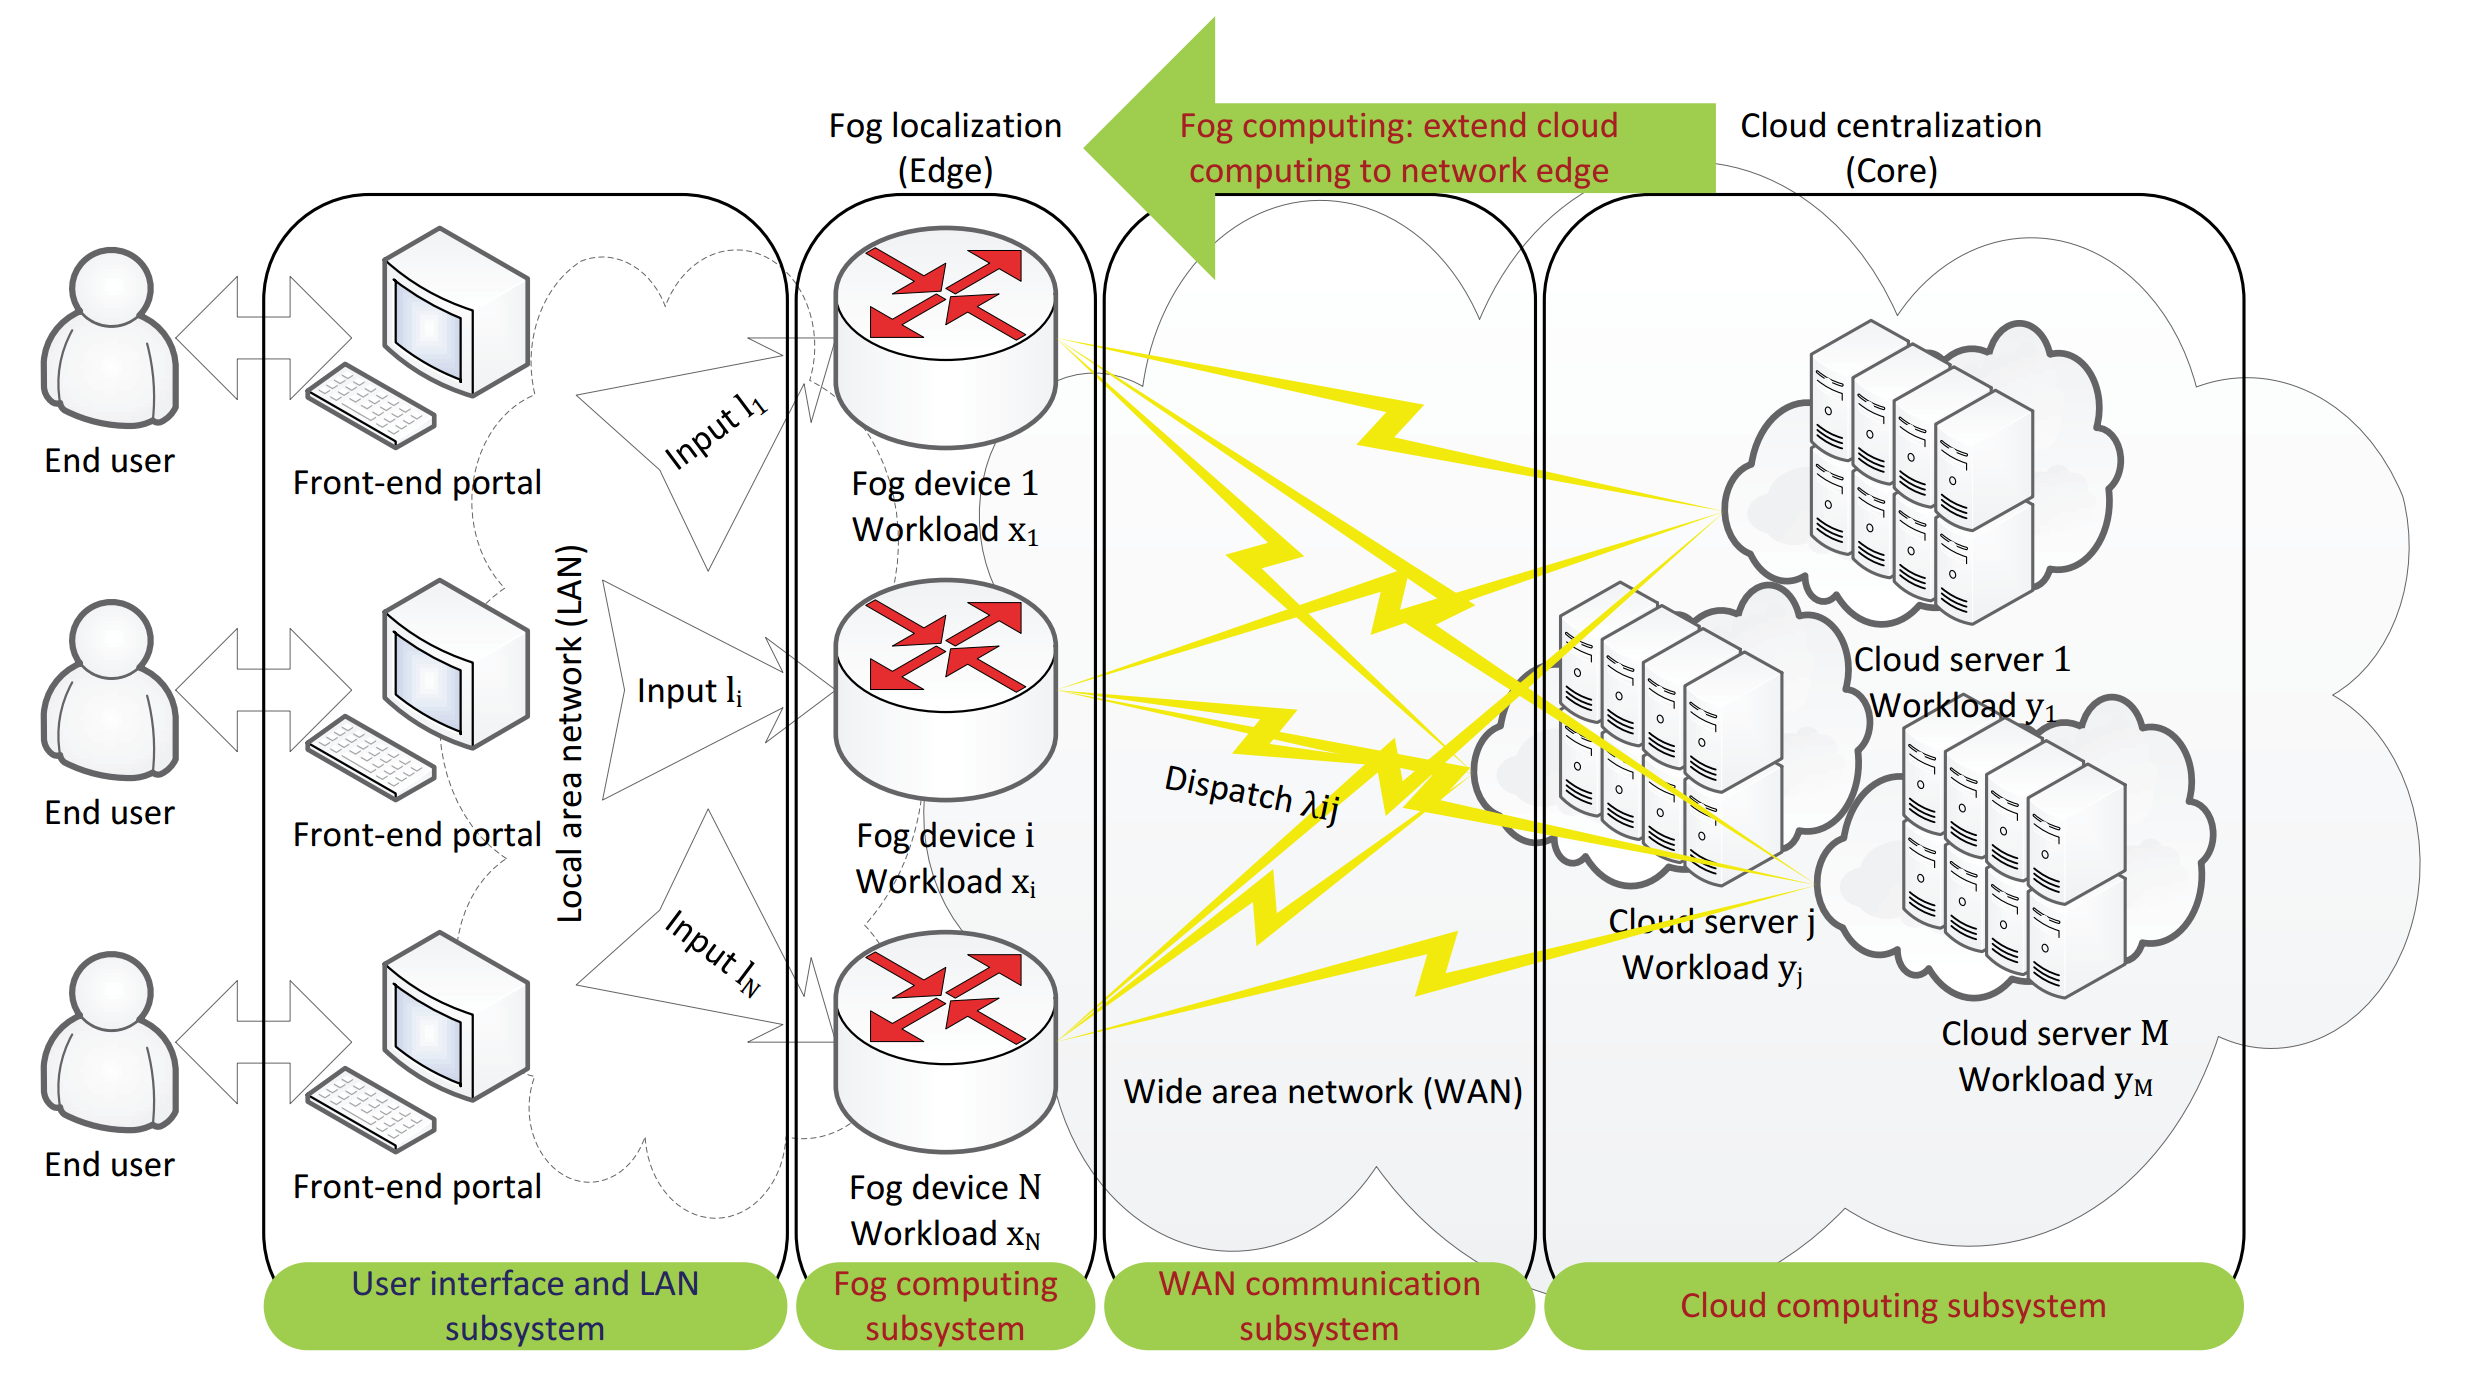
\includegraphics[width=15cm]{graphics/chapter_2/system_model_deng2016optimal}}
      \caption{مدل سیستم مقاله \cite{deng2016optimal} با چهار زیر سیستم}
      \label{fig:chapter_2:system_model_deng2016optimal}
    \end{figure}

    در \cite{barcelo2016iot} نویسندگان مسأله توزیع پردازش سرویس‌ها‌ را به صورت مسأله بهینه سازی برای کمینه کردن هزینه فرمول‌بندی کرده‌اند که با استفاده از برنامه ریزی خطی قابل حل می‌باشد.
    تمرکز آن‌ها روی مصرف انرژی است که امروزه بخش اصلی هزینه شبکه‌ها و فراهم‌کننده‌های ابری را تشکیل می‌دهد.
    آن‌ها ابتدا یک مدل ریاضی برای شبکه اینترنت اشیاء ابری ارائه می‌دهند که ظرفیت، کارایی و قابلیت اطمینان حسگر‌ها، منابع پردازشی و منابع شبکه را در محدوده دستگاه‌های انتهایی، دستگاه‌های دسترسی به شبکه و لایه ابری در نظر می‌گیرند.
    سپس هر سرویس اینترنت اشیاء را با یک گراف ریشه‌دار جهت دار مدل می‌کنند که رابطه‌ی بین تابع‌هایی که باید روی اطلاعات سرویس اجرا شوند تا نتیجه نهایی مورد دلخواه کاربر بدست بیاید را در خود نگه می‌دارد.
    \cref{fig:chapter_2:service_graph_barcelo2016iot} نمونه‌ای از این گراف را نشان می‌دهد که سه تابع $p1$، $p2$ و $p3$ باید روی داده‌های ورودی $o5$ و $o4$ اجرا بشوند تا نتیجه یا همان $o1$ تولید بشود.
    پس از آن مسئله توزیع سرویس‌های اینترنت اشیاء را برای پیدا کردن مکان اجرا شدن تابع‌های سرویس‌های اینترنت اشیاء و مسیریابی داده‌های سرویس ها در شبکه اینترنت اشیاء معرفی می‌کنند که هدف آن کمینه کردن هزینه با در نظر گرفتن نیاز کاربران است.
    آن‌ها شبکه را به صورت یک گراف مدل می‌کنند که گره‌ها منابع پردازشی و ذخیره سازی هستند و هدف پیدا کردن گره‌های مناسب برای انجام گره‌های گراف‌ سرویس‌ها است به طوری که محدودیت‌های پردازش و انتقال گره‌ها برقرار باشد.
    در انتها به بررسی مدل پیشنهادی و تاثیر پارامتر‌های مختلف پرداخته‌اند. 
    نتایج نشان می‌دهند که مدل بهینه‌سازی و راه‌حل ارائه شده استفاده قابل انعطاف از شبکه اینترنت اشیاء را برای میزبانی، مدیریت و بهینه کردن طیف وسیعی از سرویس‌های اینترنت اشیاء فراهم می‌کند.
    در مقایسه با راه حل‌های مرسوم مبتنی بر ابر، مدل ارائه شده باعث کاهش مصرف انرژی تا ۸۰٪ در کنار کاهش تاخیر سرویس‌ها می‌شود.

    \begin{figure}[h]
      \centerline{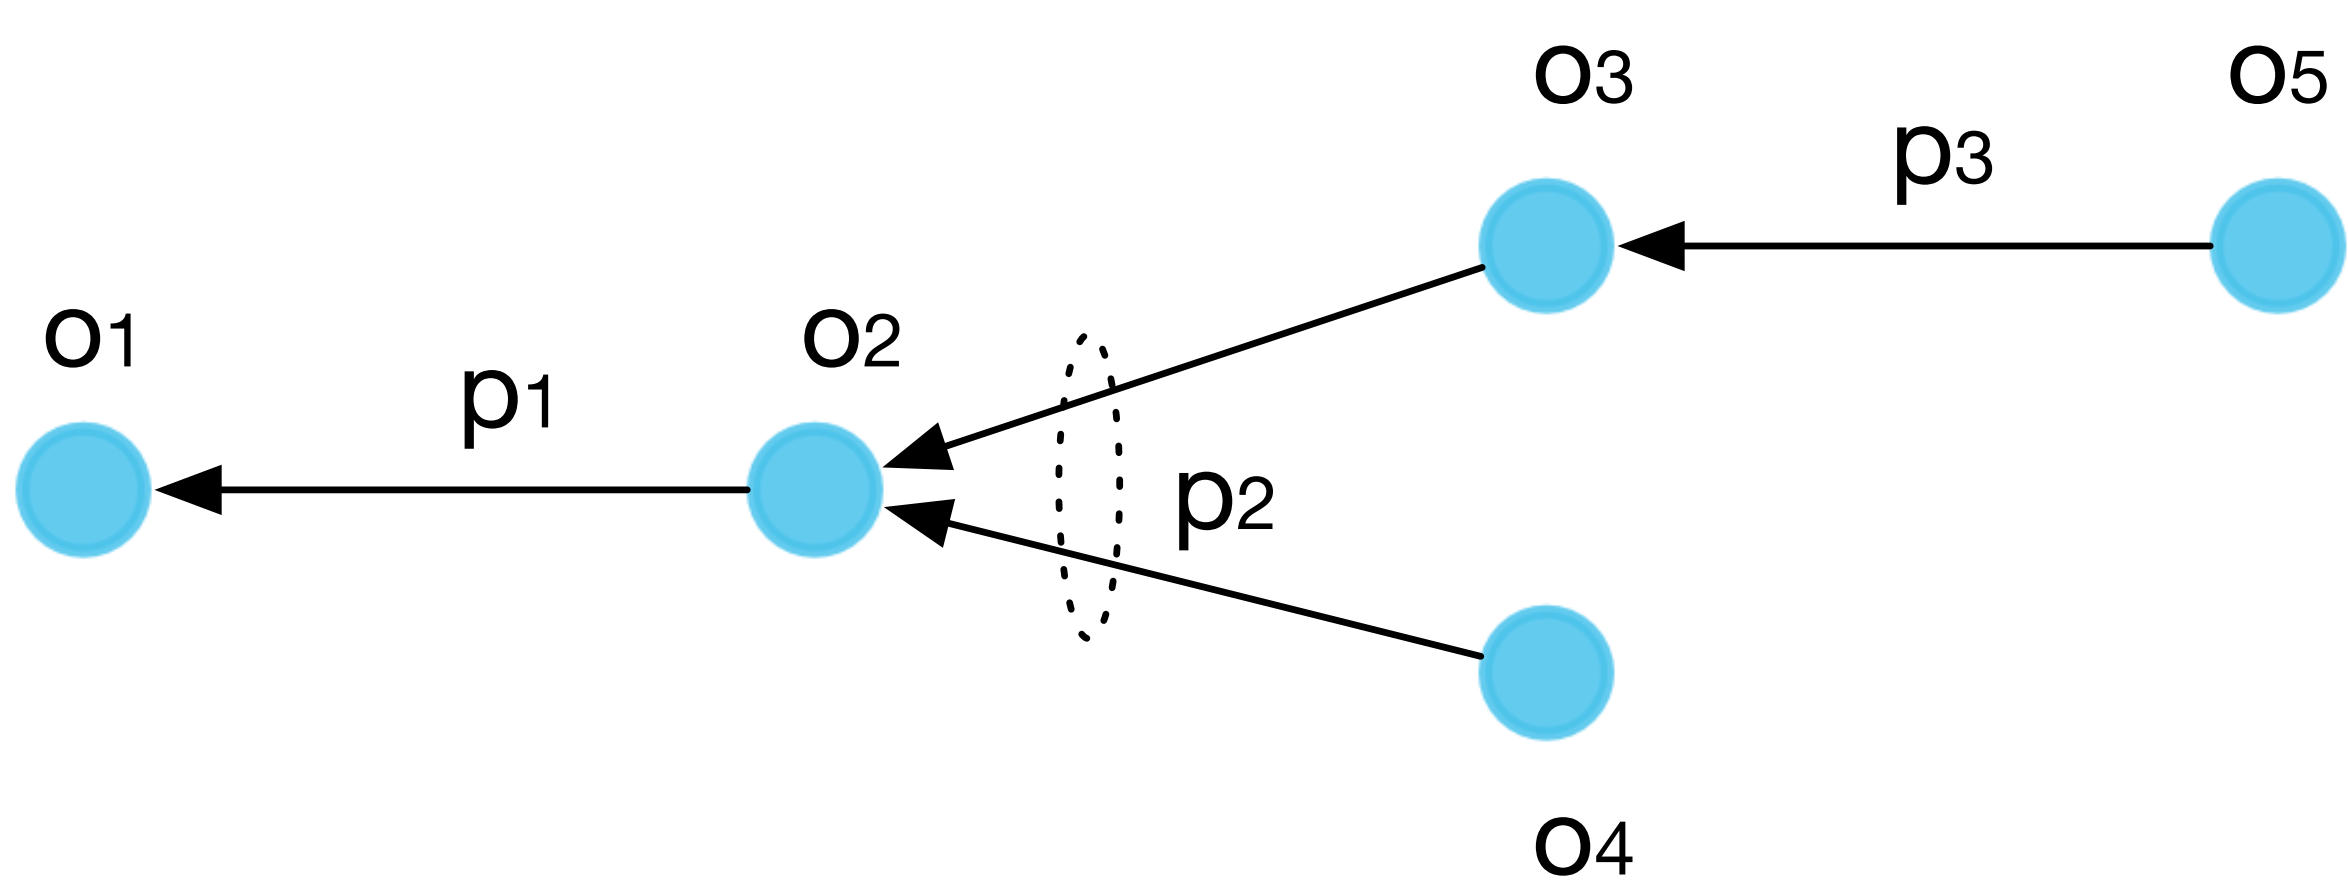
\includegraphics[width=8cm]{graphics/chapter_2/service_graph_barcelo2016iot}}
      \caption{یک گراف سرویس در \cite{barcelo2016iot}}
      \label{fig:chapter_2:service_graph_barcelo2016iot}
    \end{figure}

    \cite{zhang2017computing} به بررسی تخصیص منابع پردازشی در یک شبکه پردازش مه می‌پردازد.
    در این مقاله شبکه با سه لایه مدل می‌شود که شامل لایه‌ی گره‌های مه، لایه‌ی اپراتور‌های سرویس داده\LTRfootnote{Data Service Operator (DSO)} و لایه مشتریان سرویس‌های داده\LTRfootnote{Data Service Subscribers (DSS)} است.
    مدل سیستم ارائه شده در این مقاله در \cref{fig:chapter_2:system_model_zhang2017computing} نشان داده شده است.
    هر اپراتور سرویس داده، مجموعه‌ای از گره‌های مه را کنترل می‌کند و گره‌های مه هم سرویس‌های داده لازم را برای مشتریان فراهم می‌کنند.
    نحوه تخصیص منابع پردازشی محدود گره‌های مه به مشتریان سرویس‌های داده برای رسیدن به حالت بهینه و پایدار، یک مسئله مهم معرفی شده است.
    آن‌ها یک چهارچوب بهینه سازی مشترک بین همه‌ی اپراتور‌های سرویس‌های داده، گره‌های مه و مشتریان سرویس‌های داده ارائه می‌دهند تا به یک تخصیص منابع بهینه به صورت توزیع شده برسند.
    در این چهارچوب آن‌‌ها ابتدا از بازی استکلبرگ\LTRfootnote{Stackelberg Game} برای آنالیز مسئله قیمت گذاری برای اپراتور‌های سرویس داده و مسئله تخصیص منابع برای مشتریان سرویس‌های داده استفاده می‌کنند.
    در سناریویی که اپراتور‌های مراکز داده، میزان منابع پردازشی که مشتریان سرویس‌های داده می‌خرند را بدانند از تئوری تطبیق\LTRfootnote{Matching Theory} برای پیدا کردن ارتباط گره‌های مه و اپراتور‌های سرویس‌های داده استفاده شده است.
    در انتها در بین گره‌های مه که اپراتور سرویس‌های داده مشترکی دارند دوباره از تئوری تطبیق برای پیدا کردن ارتباط گره‌های مه و مشتریان سرویس‌های داده استفاده شده است.
    نتایج شبیه سازی نشان می‌دهند که چهارچوب ارائه شده، کارایی شبکه اینترنت اشیاء را به میزان چشمگیری افزایش می‌دهد.

    \begin{figure}[h]
      \centerline{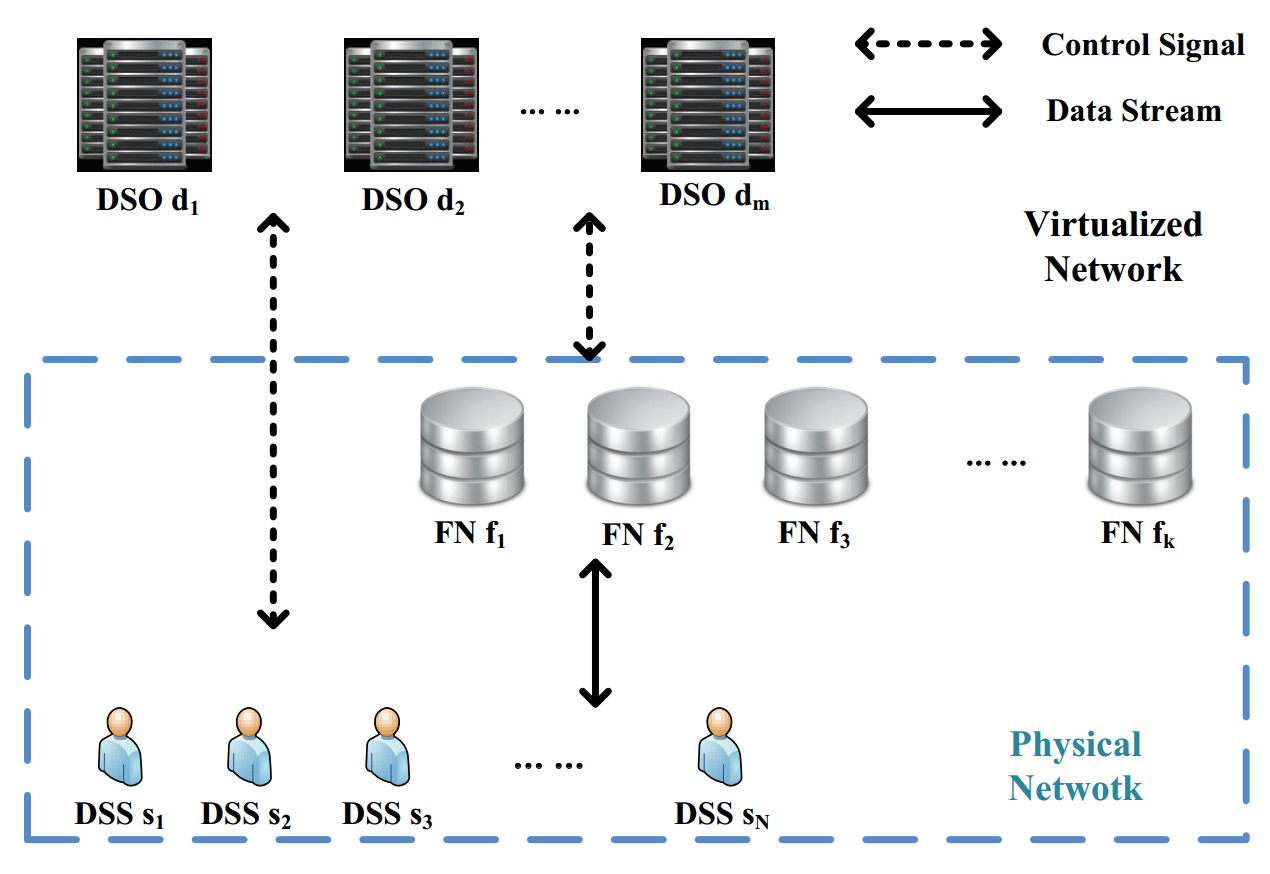
\includegraphics[width=10cm]{graphics/chapter_2/system_model_zhang2017computing}}
      \caption{مدل سیستم مقاله \cite{zhang2017computing}}
      \label{fig:chapter_2:system_model_zhang2017computing}
    \end{figure}

    در \cite{liu2017multiobjective} از پردازش مه برای کاهش بار پردازشی مراکز داده استفاده شده است.
    مسأله به صورت یک بهینه‌سازی فرمول‌بندی شده است که تلاش می‌کند، تأخیر، مصرف انرژی و هزینه را کمینه کند.
    در این مقاله، برای بررسی کامل مصرف انرژی، تاخیر و هزینه‌ی پرداختی از تئوری صف استفاده شده است.
    سه مدل مختلف صف برای دستگاه‌های لبه شبکه، گره‌های مه و مراکز داده ابری استفاده شده است و نرخ داده‌ها و مصرف انرژی اتصالات بیسیم مورد بررسی قرار گرفته‌اند.
    برای این منظور یک سیستم پردازش ابری مبتنی بر مه مورد بررسی قرار گرفته است و برای بررسی دقیق مصرف انرژی و تاخیر مدل‌های مختلف صف به اجزاء شبکه اعمال شده است.
    به صورت خاص، اتصالات بیسیم و منابع پردازشی برای مدل کردن مصرف انرژی، تاخیر و هزینه پرداختی مد نظر قرار گرفته‌اند.
    همانطور که در \cref{fig:chapter_2:system_model_liu2017multiobjective} مشخص است، در خواست‌ها برای هر کدام از منابع در صف قرار گرفته و توسط منبع مربوطه پردازش می‌شوند.
    پس از تبدیل مسئله به یک مسئله بهینه سازی با یک تابع هدف، به بررسی نتایج شبیه‌سازی پرداخته شده است.
    این شبیه‌سازی‌ها نشان می‌دهند که راه حل ارائه شده، کارایی مناسبی دارد و نسبت به راه حل‌های ارائه شده توسط دیگران مناسب‌تر است.

    \begin{figure}[h]
      \centerline{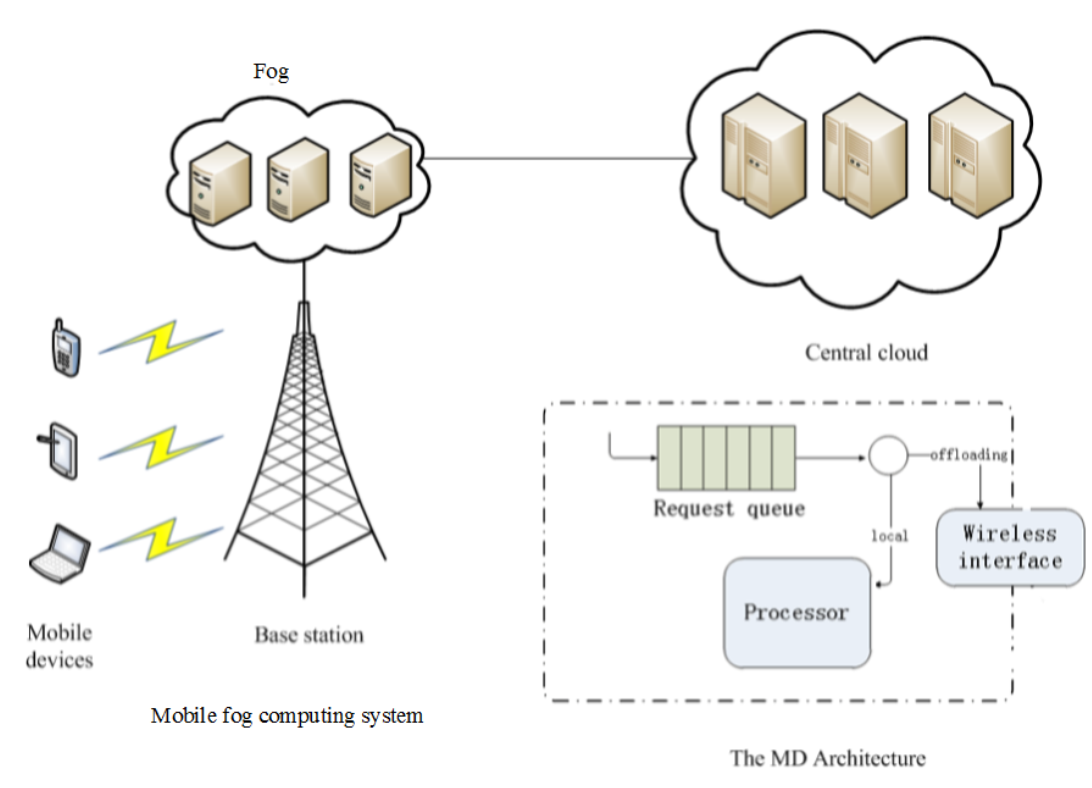
\includegraphics[width=9cm]{graphics/chapter_2/system_model_liu2017multiobjective}}
      \caption{مدل سیستم مقاله \cite{liu2017multiobjective}}
      \label{fig:chapter_2:system_model_liu2017multiobjective}
    \end{figure}

    نویسندگان در \cite{gu2018joint} مسأله‌ی تخصیص منابع رادیویی و پردازشی را بررسی کرده‌اند.
    قسمت اول \cref{fig:chapter_2:system_model_gu2018joint} مدل سیستم استفاده شده در این مقاله را نشان می‌دهد.
    در این مقاله تخصیص منابع پردازشی و رادیویی به صورت همزمان مورد مطالعه قرار گرفته است تا کارایی سیستم را بهینه کند و رضایت کاربران را افزایش دهد.
    عوامل مهمی مانند تاخیر، کیفیت ارتباطات و نیاز کاربران در نظر گرفته شده است.
    در این مقاله کاربران نیاز خود را در قالب تاخیر و اندازه داده‌ها به فراهم کنندگان ابری اعلام می‌کنند.
    فراهم کنندگان ابری با ارتباط با کاربران سعی در پیدا کردن گره‌های مه مناسب می کنند تا پردازش‌های مورد نیاز کاربران را به همراه تخصیص طیف رادیویی به آن‌ها انتقال بدهند.
    برای بیشینه کردن رضایت کاربران، مسأله به صورت یک مسأله برنامه‌ریزی غیرخطی عدد صحیح مخلوط فرمول بندی شده است.
    در فرمول‌بندی محدودیت‌هایی مانند تاخیر سرویس‌ها، کیفیت انتقال، کنترل توان و غیره در نظر گرفته شده‌است.
    از بازی تخصیص پروژه به دانش آموزان در تئوری تطبیق برای پیدا کردن تخصیص منابع بهینه استفاده شده است.
    در این بازی، تعدادی پروژه وجود دارد و دانش آموزان می‌توانند لیستی از پروژه‌های مورد علاقه خود را انتخاب کنند.
    در نهایت مربی پروژه‌ها را به دانش آموزان اختصاص می‌دهد به طوری که رضایت همه دانش آموزان از پروژه اختصاص یافته به خود بیشینه باشد.
    همانطور که در قسمت دوم \cref{fig:chapter_2:system_model_gu2018joint} مشخص است در این جا فراهم کننده‌های ابری به عنوان مربی و منابع پردازشی و رادیویی به عنوان پروژه‌ها و کاربران به عنوان دانش آموزان مدل شده‌اند.
    با ارائه استراتژی‌هایی، تاثیر انتخاب بازیگران بر یکدیگر حذف و رسیدن به یک تعادل پایدار تضمین شده و کارایی سیستم بهبود یافته است.
    نتایج شبیه‌سازی‌های ارائه شده هم نمایان‌گر کارایی نزدیک به بهینه از دید کاربران و سیستم می باشد.

    \begin{figure}[h]
      \centerline{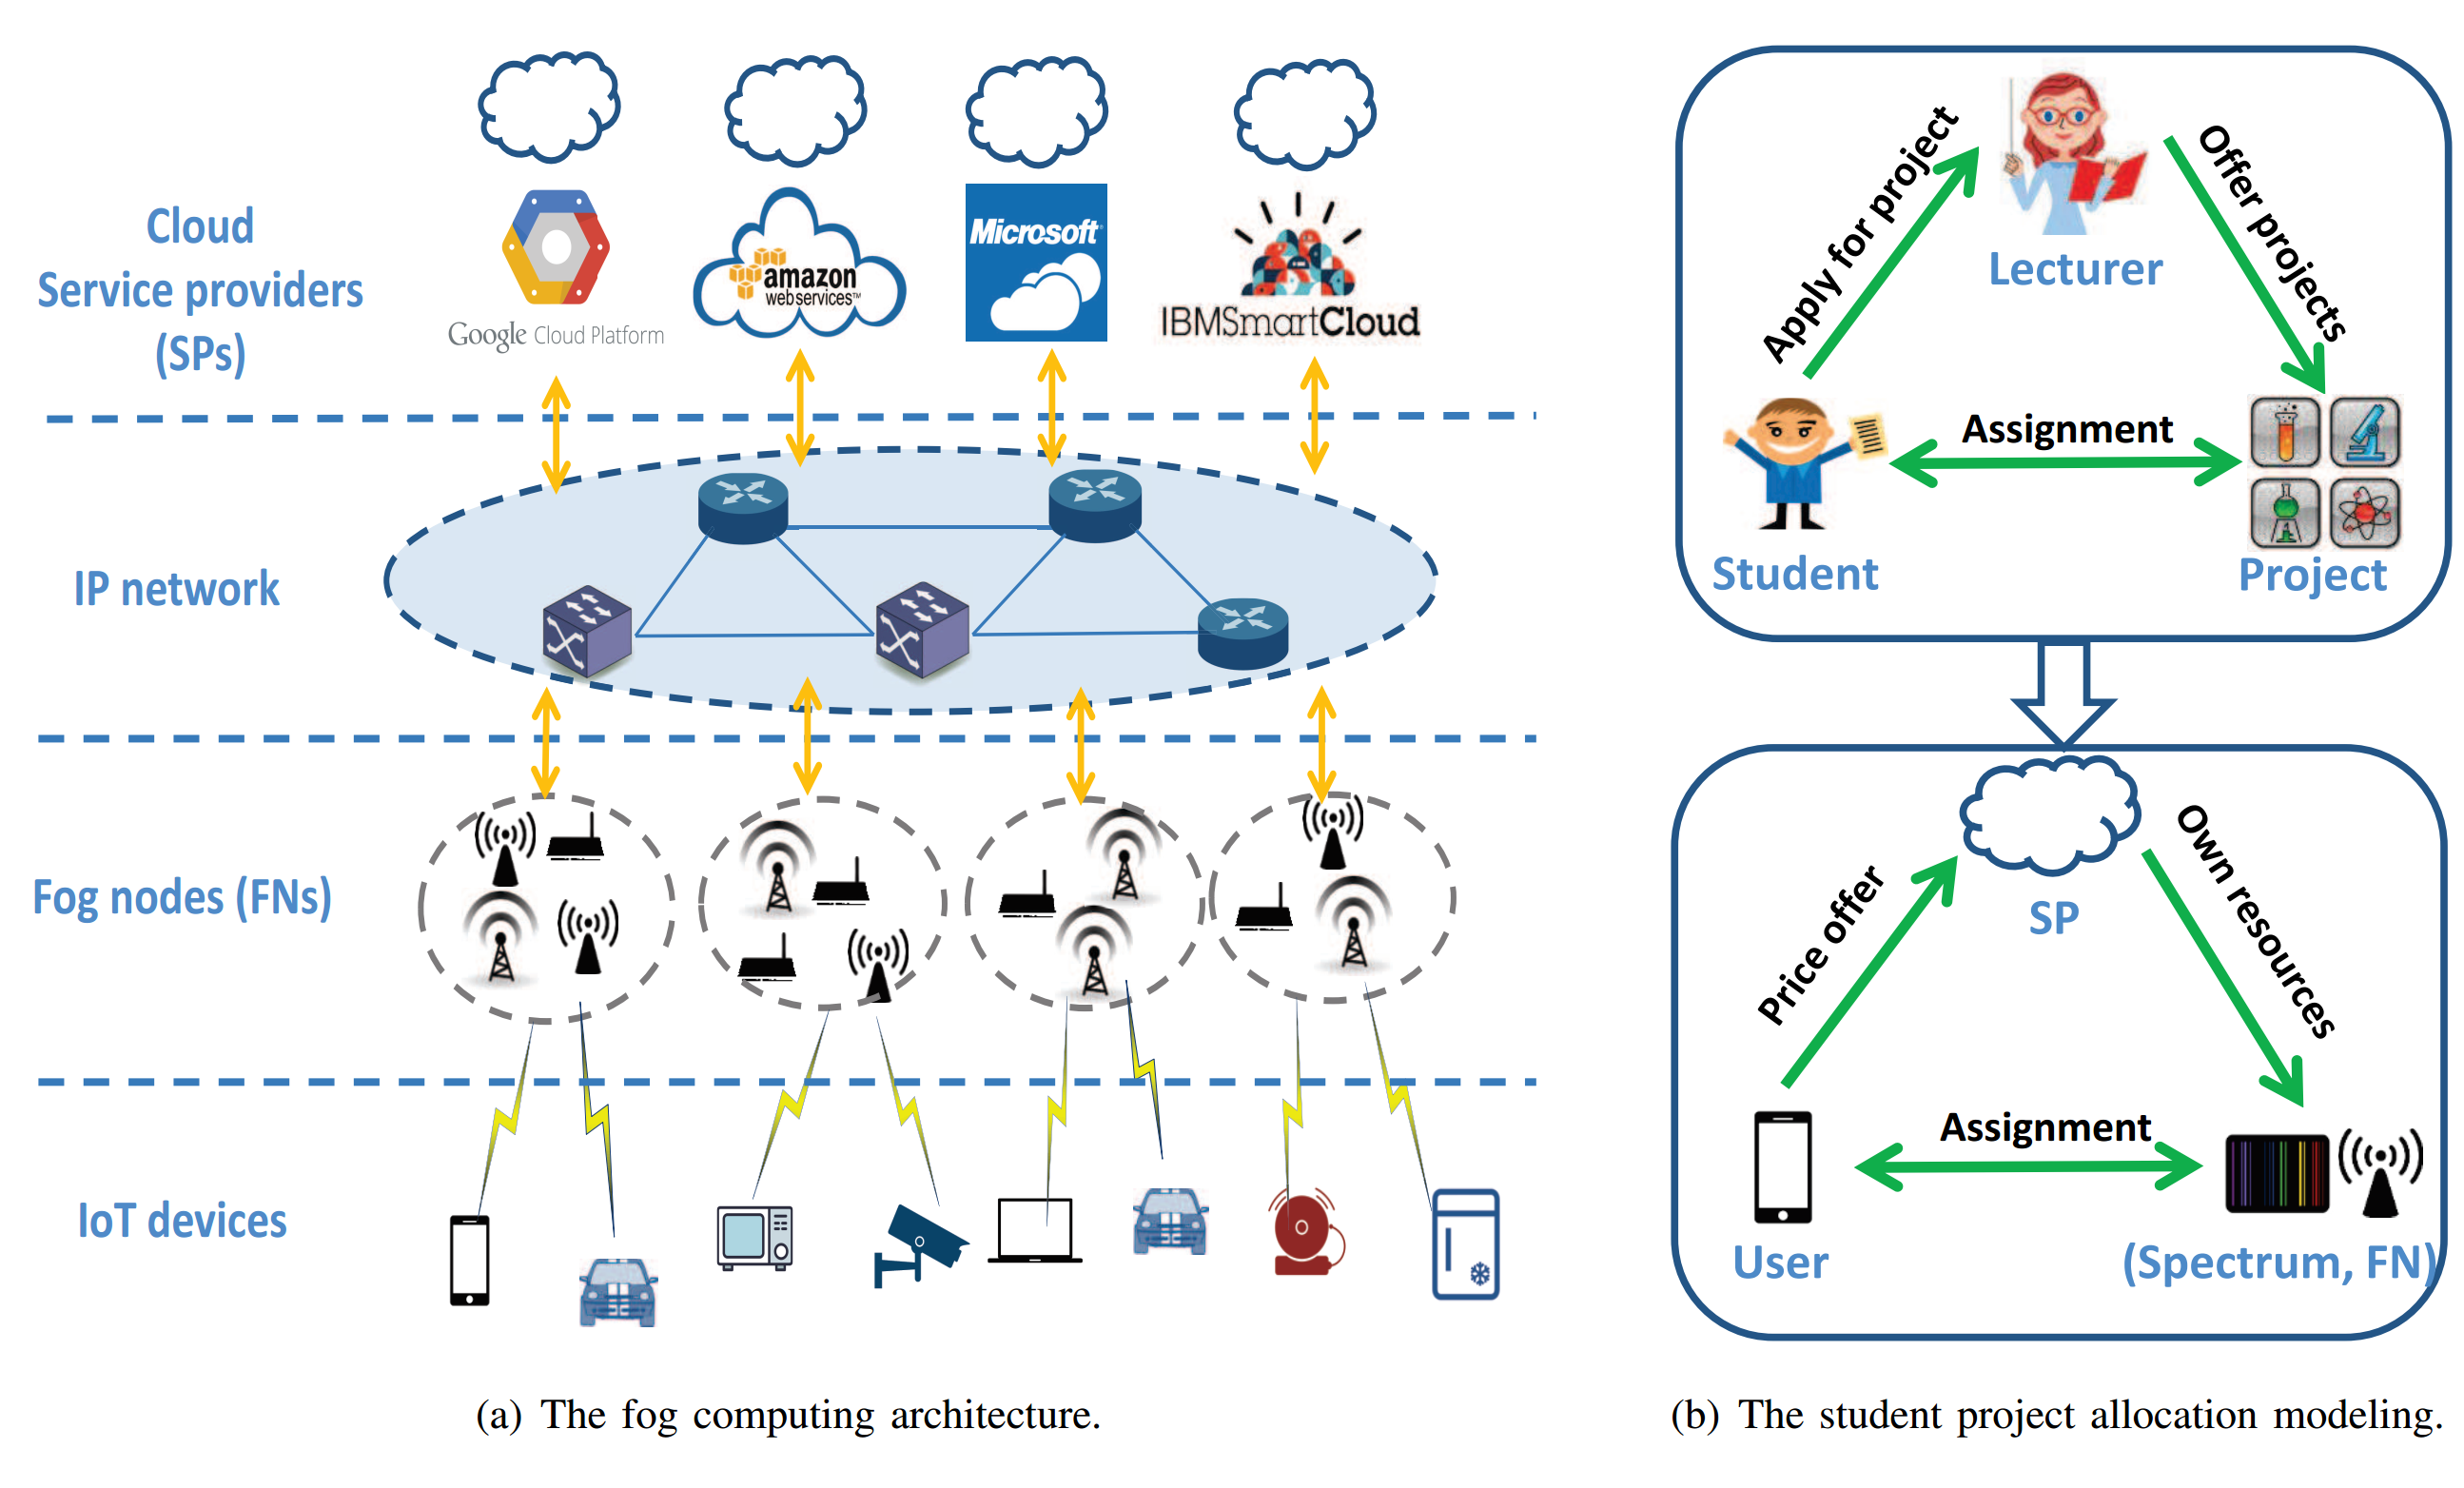
\includegraphics[width=12cm]{graphics/chapter_2/system_model_gu2018joint}}
      \caption{مدل سیستم مقاله \cite{gu2018joint}}
      \label{fig:chapter_2:system_model_gu2018joint}
    \end{figure}

    مقاله \cite{du2018computation} به بررسی مسئله تخصیص منابع پردازشی به همراه توان ارسالی و پهنای‌باند رادیویی می‌پردازد به طوری که عدالت بین کاربران و حداکثر تاخیر قابل تحمل رعایت شود.
    این مسئله بهینه سازی به صورت کمینه کردن بیشینه هزینه وزن دار فرمول بندی شده است و هزینه شامل تاخیر و انرژی مصرفی بین همه کاربران است.
    بهینه سازی ارائه شده یک مسئله برنامه‌ریزی غیرخطی عدد صحیح مخلوط است که به سختی قابل حل است و برای حل آن یک الگوریتم با پیچیدگی کم ارائه شده است.
    برای این کار مسئله ابتدا به یک مسئله QCQP\LTRfootnote{Quadratically Constrained Quadratic Programming} تبدیل می‌شود.
    سپس با استفاده از برنامه‌ریزی کسری\LTRfootnote{Fractional Programming} مسئله به یک بهینه سازی محدب تبدیل می‌شود.
    نتایج شبیه‌سازی‌های ارائه شده نشان دهنده مناسب بودن همگرایی الگوریتم ارائه شده و عدالت بین کاربران و کارایی در زمینه تاخیر و انرژی مصرفی حاصل از آن در برابر الگوریتم‌های موجود می‌باشد.

    در مقاله \cite{zhu2018folo} نویسندگان به ارائه چهارچوبی برای بهینه سازی تاخیر و کیفیت تخصیص وظایف پردازشی در پردازش مه خودرو‌ها می‌پردازند.
    چهارچوب ارائه شده، تحرک خودرو‌ها که شامل خودرو‌هایی که نیاز به پردازش وظایف دارند و خودرو‌هایی که به عنوان گره‌های مه عمل می‌کنند را شامل می‌شود.
    مدل سیستم این مقاله در \cref{fig:chapter_2:system_model_zhu2018folo} نشان داده شده است.
    خودرو‌های دارای وظیفه‌ی پردازشی و خودرو‌های گره‌های مه در شکل مشخص هستند.
    مسئله تخصیص وظایف به صورت یک مسئله بهینه سازی معرفی شده و تابع هدف آن شامل تاخیر و کیفیت است.
    مانند بقیه مقاله‌ها، مسئله ارائه شده در این مقاله هم نیاز به زمان زیادی برای حل دارد و به همین دلیل مقاله یک الگوریتم مبتنی بر برنامه ریزی خطی برای حل آن ارائه کرده است.
    نتایج شبیه سازی‌های ارائه شده در این مقاله نشان می‌دهند که چهارچوب ارائه شده نسبت به روش تخصیص وظایف تصادفی، تاخیر را تا ۲۷٪ و کیفیت را تا ۵۶٪ بهبود می‌بخشد.

    \begin{figure}[h]
      \centerline{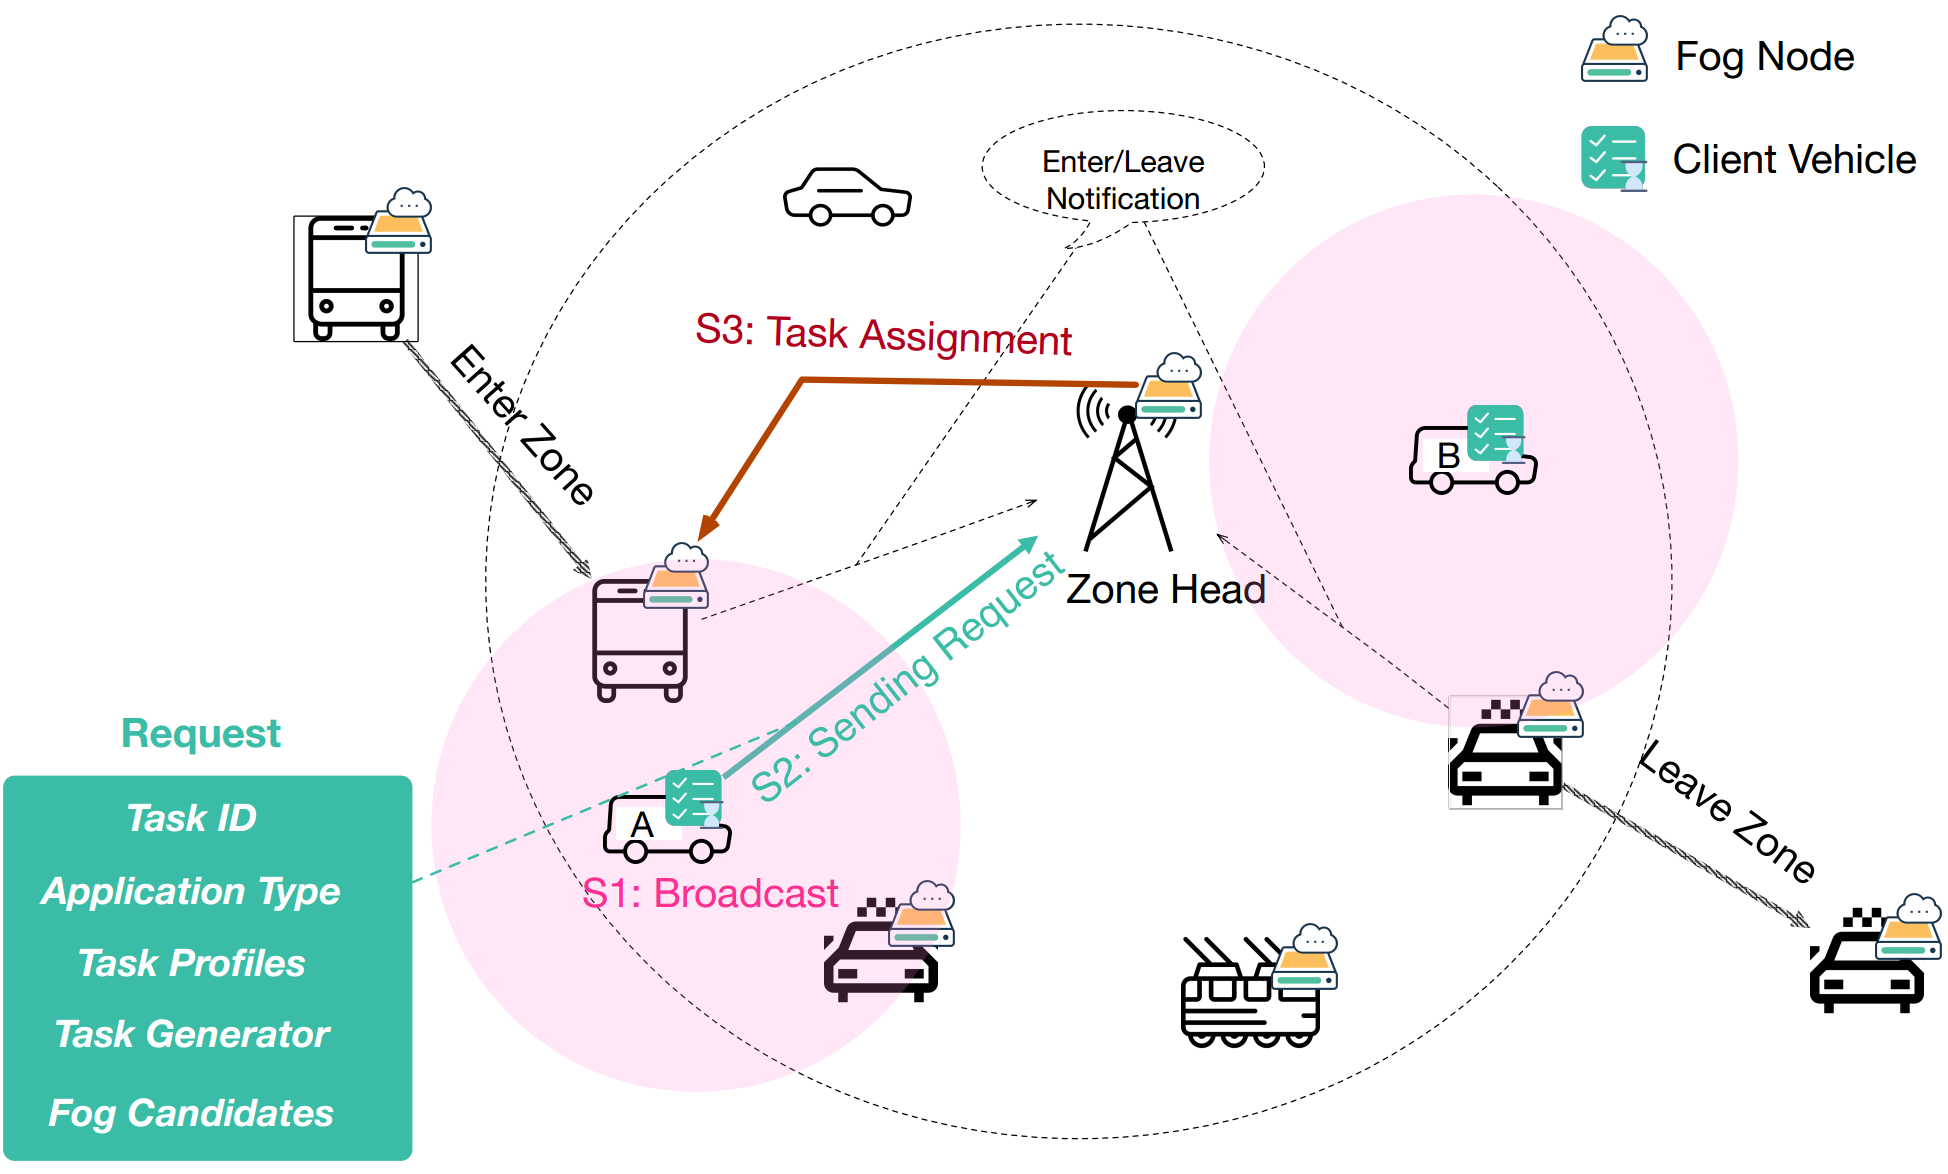
\includegraphics[width=9.2cm]{graphics/chapter_2/system_model_zhu2018folo}}
      \caption{مدل سیستم مقاله \cite{zhu2018folo}}
      \label{fig:chapter_2:system_model_zhu2018folo}
    \end{figure}

    مقاله \cite{zhou2018computation} به استفاده از هواپیما‌های بدون سرنشین \LTRfootnote{Unmanned Aerial Vehicle} در پردازش لبه می‌پردازد.
    \cref{fig:chapter_2:system_model_zhou2018computation} مدل سیستم این مقاله را نشان می‌دهد.
    در این مقاله کاربران باید تصمیم بگیرند که پردازش اطلاعات توسط خودشان انجام شود یا از هواپیمای بدون سرنشین که پردازنده قدرتمندی دارد استفاده کنند.
    مسئله بیشینه کردن نرخ پردازش در دو حالت کلی و جزئی با محدودیت‌های انرژی و سرعت حرکت این پرنده‌ها در نظر گرفته شده است.
    مانند باقی مقاله‌ها برای حل مسئله در زمان مناسب، یک الگوریتم دو مرحله‌ای و یک الگوریتم سه مرحله‌ای ارائه شده است.
    نتایج شبیه‌سازی‌های ارائه شده نشان می‌دهند که روش تخصیص منابع ارائه شده بهبود قابل توجهی نسبت به سایر روش‌ها دارد.
    همچنین پیچیدگی محاسباتی و همگرایی سریع از دیگر مزایای روش ارائه شده می‌باشند.

    \begin{figure}[h]
      \centerline{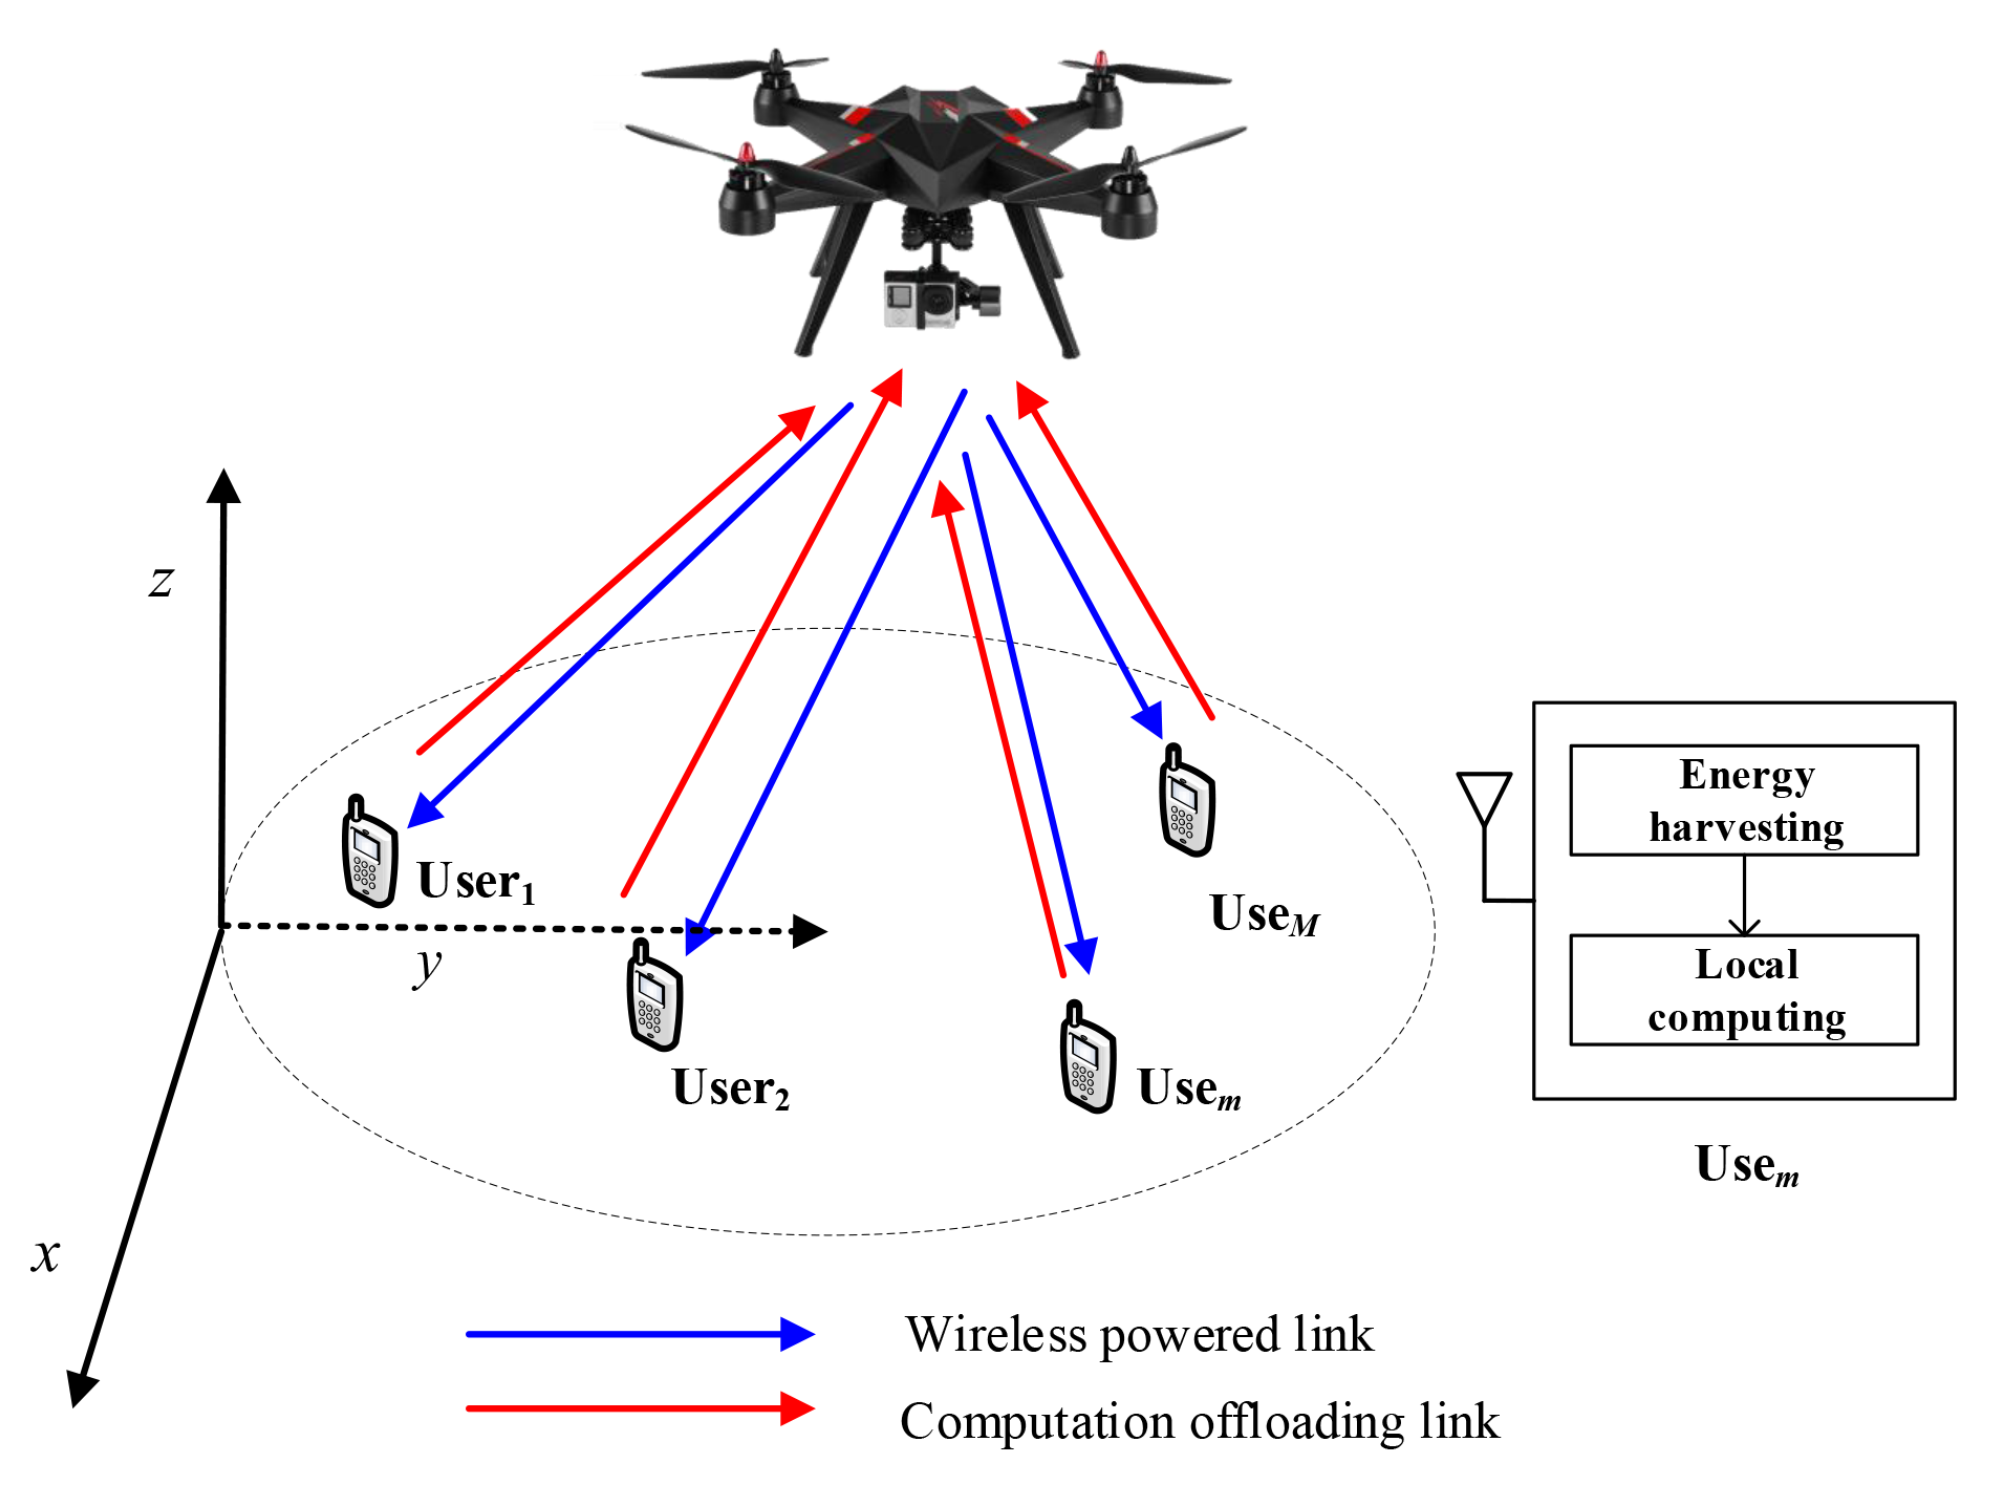
\includegraphics[width=10cm]{graphics/chapter_2/system_model_zhou2018computation}}
      \caption{مدل سیستم مقاله \cite{zhou2018computation}}
      \label{fig:chapter_2:system_model_zhou2018computation}
    \end{figure}

    در \cite{wang2019smart} نویسندگان یک روش تخصیص منابع مبتنی بر یادگیری تقویتی عمیق\LTRfootnote{Deep Reinforcement Learning} ارائه داده‌اند.
    الگوریتم ارائه شده شامل مسیریابی (تخصیص منابع شبکه) و تخصیص منابع پردازشی در شبکه پردازش لبه متحرک است.
    با اعمال تکنولوژی‌های شبکه‌های نرم‌افزاری در مدل ارائه شده، از مزایای آن مانند کنترل متمرکز زیرساخت شبکه بهره‌مند شده اند.
    در این مقاله تاخیر مسیریابی شبکه و تاخیر پردازشی به عنوان تاخیر سرویس در نظر گرفته شده‌اند و هدف مقاله کمینه کردن تاخیر به همراه ایجاد تعادل در استفاده از منابع پردازشی و منابع شبکه است.
    نتایج شبیه سازی‌های بررسی شده نشان می‌دهند که راه حل ارائه شده بهتر از روش‌های که قبلا برای این مسئله ارائه شده‌اند عمل می‌کند.
